The rise of voice-based interfaces is really impressive over the last couple of years. They are not only integrated to mobile device (Apple Siri, Google Assitant) but also deployed to entire voice-first device (Amazon Echo, Google Home). According to VoiceLabs's report \cite{VoiceLabs:2017}, there were 1.7 million voice-first devices shipped in 2015. In 2016, this figure were 6.5 million and is predicted to be 24.5 million this year. The potential to build application on top of these interfaces seems limitless. We can directly use voice to order the device to play music, read newspaper, turn on/off light etc. My project is focused on robotic applications, specially for remote movement control and object finding. The objective is to build a voice system that listens to user's commands, transfers these audio signals to text, extracts the information from text and maps to corresponding robot actions (figure \ref{fig:diagramSystem}). 
\begin{figure}[tb]
\centering
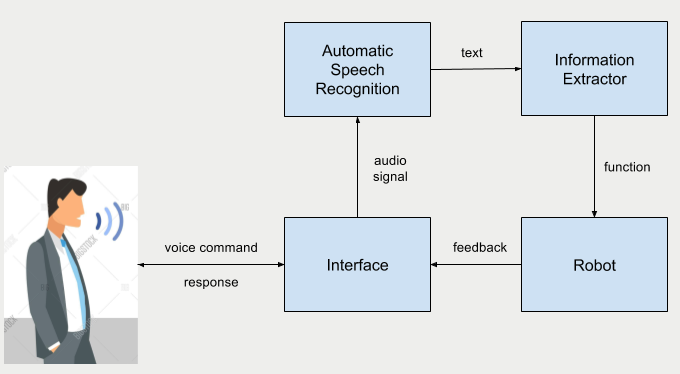
\includegraphics[width = 0.7\hsize]{./figures/diagramSystem}
\caption{Diagram of the system}
\label{fig:diagramSystem}
\end{figure}


%Two closely related reasons for this booming era of voice-based system is the success of Deep Neural Network along with the availibility of Big Data. 
%
%Deep Neural Network (DNN) is a machine learning method that was introduced in second half of 20th century. Because of its massive computation demand, DNN was not successful until 2012, when strong GPU and big data are available. Previously, traditional methods of speech recognition and speech synthesis based on Gaussian Mixture and Hidden Markov models involve many non-uniform internal-handcrafting rules 
%
%have been taken over by DNN